\documentclass{beamer}
 
\usepackage[utf8]{inputenc}


\usetheme{Madrid}
\usecolortheme{default}
\usepackage{caption}
\usepackage{subcaption}


\usepackage{physics}
\usepackage{amsmath}
\usepackage{amsfonts}
\usepackage{esint}
\usepackage{bbold}
\usepackage{mathtools}
\usepackage{dsfont}
\usepackage{amsthm}
\usepackage{bbm}
\usepackage{amssymb}
\theoremstyle{definition}
\newtheorem{defn}{Definition}[section]
\newtheorem{prop}{Properties}[section]
\newtheorem{rmk}{Remark}[section]
\newtheorem{exmp}{Example}[section]
\newtheorem{prob}{Problem}[section]
\newtheorem{proposition}{Proposition}
\newtheorem{thm}{Theorem}[section]
\newtheorem*{prob*}{Problem}
\newtheorem*{sln*}{Solution}
\usepackage{empheq}
\usepackage{tensor}
\usepackage{hyperref}
\usepackage{xcolor}

\newcommand{\R}{\mathbb{R}}
\newcommand{\F}{\mathcal{F}}
\newcommand{\p}{\partial}

\newcommand{\V}{\mathbf{V}}
\newcommand{\W}{\mathbf{W}}
\newcommand{\Z}{\mathbf{Z}}
\newcommand{\Y}{\mathbf{Y}}
\newcommand{\U}{\mathbf{U}}
\newcommand{\X}{\mathbf{X}}

\newcommand{\A}{\mathcal{A}}
\newcommand{\B}{\mathcal{B}}

\newcommand{\xpan}{\text{span}}

\newcommand{\lag}{\mathcal{L}}

\newcommand{\J}{\mathbf{J}}

\newcommand{\M}{\mathcal{M}}

\newcommand{\lp}{\left(}
\newcommand{\rp}{\right)}

\newcommand{\lb}{\left[}
\newcommand{\rb}{\right]}

\newcommand{\lc}{\left\{}
\newcommand{\rc}{\right\}}

\newcommand{\K}{\mathcal{K}}

\newcommand{\N}{\mathcal{N}}

\newcommand{\E}{\mathcal{E}}

\newcommand{\ima}{\text{Im}}
\newcommand{\lin}{\overset{\text{linear}}{\longrightarrow}}
\newcommand{\T}{\mathcal{T}}
\newcommand{\poly}{\mathbb{P}}
\newcommand{\s}{\mathcal{S}}

\newcommand{\gives}{\rotatebox[origin=c]{180}{$\Rsh$}	}


\newcommand{\bigzero}{\mbox{\normalfont\Large\bfseries 0}}
\newcommand{\rvline}{\hspace*{-\arraycolsep}\vline\hspace*{-\arraycolsep}}




 
 
%Information to be included in the title page:
\title[A generalized integration formula...]
{
	Convolution powers
	of complex-valued functions on $\mathbb{Z}^d$
}



\author[Bui \& Randles] % (optional)
{Huan Q. Bui \\
	\& \\
	Professor Evan Randles}

\institute[Colby College] % (optional)
{
}
\date{CLAS, April 28, 2021}
 
%\logo{
\includegraphics[height=0.3cm]{colby.png}}
 
\begin{document}
 
\frame{\titlepage}



%%%%%%%%%%%%%%%%%%%%%%%%%%%%%%%%%%%%%%%%%%%%%%%%%%%%%%%%%%%%%%%%%%%%%%%%%

 
%\begin{frame}
%\frametitle{Layout}
%\tableofcontents
%\end{frame}

%%%%%%%%%%%%%%%%%%%%%%%%%%%%%%%%%%%%%%%%%%%%%%%%%%%%%%%%%%%%%%%%%%%%%%%%%


\section{The Classical Local Limit Theorem}
\begin{frame}
\frametitle{The Classical Local Limit Theorem}

Given iid random vectors $X_1, X_2, \dots, X_n \in \mathbb{Z}^d$ from a probability distribution $\phi$:
\begin{equation*}
\phi(x) = \mathbb{P}(X_i = x).
\end{equation*}




The random walk $S_n = X_1 + X_2 + \dots X_n$ has distribution
\begin{equation*}
\phi^{(n)}(x)=\sum_{y\in\mathbb{Z}^d}\phi^{(n-1)}(x-y)\phi(y) = \phi^{(n-1)}\ast \phi^{(1)}.
\end{equation*}

\textbf{How does $\phi^{(n)}$ behave when $n\to \infty$?}

\end{frame}




\begin{frame}
%\frametitle{The Classical Local Limit Theorem}
\noindent \underline{Example:} Simple random walk in $\mathbb{Z}^2$

\begin{figure}
	\begin{subfigure}{0.49\textwidth}
		\centering
		\includegraphics[width=0.8\textwidth]{convolve_1.eps}
	\end{subfigure}
	\begin{subfigure}{0.49\textwidth}
		\centering
		\includegraphics[width=0.8\textwidth]{convolve_2.eps}
	\end{subfigure}
\end{figure}
\vspace{-15pt}
\begin{figure}
	\begin{subfigure}{0.49\textwidth}
		\centering
		\includegraphics[width=0.8\textwidth]{convolve_11.eps}
	\end{subfigure}
	\begin{subfigure}{0.49\textwidth}
		\centering
		\includegraphics[width=0.8\textwidth]{convolve_22.eps}
	\end{subfigure}
\end{figure}


\end{frame}





\begin{frame}
\frametitle{The Classical Local Limit Theorem}
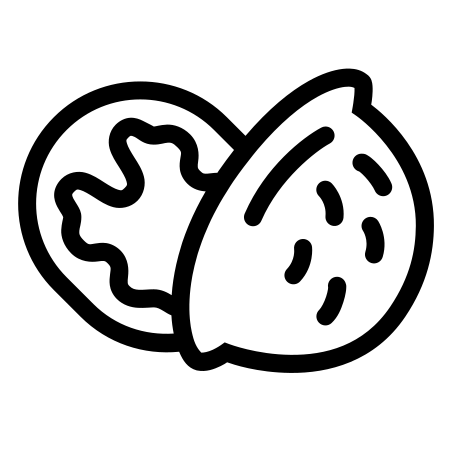
\includegraphics[scale=0.025]{nutshell} If $\phi$ is a ``nice'' probability distribution on $\mathbb{Z}^d$ with finite variance then 
%\pause 
\begin{itemize}
	\item Global decay: There are positive constants $C_1, C_2$ for which 
	\begin{equation*}
	C_1 n^{-d/2} \leq \| \phi^{(n)} \|_\infty \leq C_2n^{-d/2}, \quad \forall n\in \mathbb{N}_+.
	\end{equation*}
	%\pause
	
	
	\item Local description for large $n$:
	\begin{equation*}
	\phi^{(n)}(x) = n^{-d/2} \Phi_\phi \lp x n^{-d/2} \rp + o\lp n^{-d/2} \rp, \quad \text{	uniformly for } x\in \mathbb{Z}^d
	\end{equation*}
	where $\Phi_\phi$ is the generalized Gaussian associated with $\phi$. 
	%\pause
	
	\item Global estimate: There are positive constants $C$ and $M$ for which
	\begin{equation*}
	\phi^{(n)}(x) \leq \frac{C}{n^{d/2}} \exp \lp -\frac{M\abs{x}^2}{n} \rp, \quad \forall x\in \mathbb{Z}^d, n\in \mathbb{N}_+
	\end{equation*}
	
\end{itemize}
\end{frame}



\section{Beyond the Classical LLT}
\begin{frame}
\frametitle{Beyond the Classical LLT}
\textbf{What if positivity is dropped?}\\
$\,$\\

Consider $\phi: \mathbb{Z}^d \to \mathbb{C}$ and define 

\begin{equation*}
\phi^{(n)}(x)=\sum_{y\in\mathbb{Z}^d}\phi^{(n-1)}(x-y)\phi(y) = \phi^{(n-1)}\ast \phi^{(1)}.
\end{equation*}

%
%\begin{equation*}
%\| \phi \|_1 = \sum_{x\in \mathbb{Z}^d} \abs{\phi(x)} < \infty.
%\end{equation*}


About the asymptotic behavior of $\phi^{(n)}$ as $n\to \infty$, can we still ask for
\begin{itemize}
	\item A global decay?
	\item A local description?
	\item A global estimate?
\end{itemize}



\end{frame}

















\begin{frame}
\frametitle{Beyond the Classical LLT}

\underline{Example:} Look at $\phi^{(n)}$ for 
\begin{equation*}
\phi(x,y) = 
\frac{1}{768}\times
\begin{cases}
602 - 112i &(x,y) = (0,0)\\
56 + 32i   &(x,y) = (-1,0)\\
72 + 32i   &(x,y) = (1,0)\\
-16        &(x,y) = (\pm 2,0)\\
56 + 32i   &(x,y) = (0,\pm 1)\\
-28 - 8i   &(x,y) = (0,\pm 2)\\
56         &(x,y) = (0,\pm 3)\\
-1         &(x,y) = (0,\pm 4)\\
4          &(x,y) = (-1,\pm 1)\\
-4         &(x,y) = (1,\pm 1)\\
0          &\text{otherwise}.
\end{cases}
\end{equation*}
\end{frame}







\begin{frame}
\frametitle{Beyond the Classical LLT}

\begin{figure}
	\begin{subfigure}{0.495\textwidth}
		\centering
		\includegraphics[width=\textwidth]{conv_ex0.eps}
	\end{subfigure}
	\begin{subfigure}{0.495\textwidth}
		\centering
		\includegraphics[width=\textwidth]{conv_ex1.eps}
	\end{subfigure}
\end{figure}
\end{frame}



\begin{frame}
\frametitle{Beyond the Classical LLT}



\underline{Example}:

\begin{equation*}
\phi(x,y) =
\frac{1}{192}\times
\begin{cases}
144 - 64i &(x,y) = (0,0)\\
16 + 16i &(x,y) = (\pm 1, 0)\mbox{ or }(0,\pm 1)\\
-4        &(x,y) = (\pm 2,0)\mbox{ or }(0,\pm 2)\\
i   &(x,y) = \pm(1,1)\\
-i   &(x,y) = \pm(1,-1)\\
0& \text{otherwise}.
\end{cases}
\end{equation*}

\end{frame}



\begin{frame}
\frametitle{Beyond the Classical LLT}


\begin{figure}[!htb]
\begin{subfigure}{0.495\textwidth}
	\centering
	\includegraphics[width=\textwidth]{Real_400.eps}
\end{subfigure}
\begin{subfigure}{0.495\textwidth}
	\centering
	\includegraphics[width=\textwidth]{Real_1500.eps}
\end{subfigure}
\end{figure}


\end{frame}



\begin{frame}
\frametitle{Beyond the Classical LLT}

\begin{figure}[!htb]
	\begin{subfigure}{0.495\textwidth}
		\centering
		\includegraphics[width=\textwidth]{Abs_400.eps}
	\end{subfigure}
	\begin{subfigure}{0.495\textwidth}
		\centering
		\includegraphics[width=\textwidth]{Abs_1500.eps}
	\end{subfigure}
\end{figure}

%\pause 


\end{frame}


\begin{frame}
\frametitle{Beyond the Classical LLT}
\textbf{What if positivity is dropped?}\\
$\,$\\

Consider $\phi: \mathbb{Z}^d \to \mathbb{C}$ and define 

\begin{equation*}
\phi^{(n)}(x)=\sum_{y\in\mathbb{Z}^d}\phi^{(n-1)}(x-y)\phi(y) = \phi^{(n-1)}\ast \phi^{(1)}.
\end{equation*}

%
%\begin{equation*}
%\| \phi \|_1 = \sum_{x\in \mathbb{Z}^d} \abs{\phi(x)} < \infty.
%\end{equation*}


About the asymptotic behavior of $\phi^{(n)}$ as $n\to \infty$, can we still ask for
\begin{itemize}
	\item \textcolor{purple}{\textbf{A global decay? $\impliedby$}} 
	\item A local description?
	\item A global estimate?
\end{itemize}



\pause

\centering{\textbf{\textcolor{purple}{HOW?}}}


\end{frame}







\begin{frame}
\frametitle{Global decay estimate for $\abs{\phi^{(n)}}$}



\begin{center}
\fbox{{{FT\{$\phi^{(n)}$\} = (FT\{$\phi$\})$^n$}}}
\end{center}
$\,$\\


Define the Fourier transform for $\phi$ in $\mathcal{S}_d$:
\begin{equation*}
\widehat{\phi}(\xi)=\sum_{x\in\mathbb{Z}^d}\phi(x)e^{ix\cdot\xi}
\end{equation*}
$\,$\\
The asymptotic behavior of $\phi^{(n)}$ is characterized by how $\widehat{\phi}$ behaves near where $|\widehat{\phi}|$ is maximized:

\begin{equation*}
\Omega(\phi)=\left\{\xi\in \mathbb{T}^d:\abs{\widehat{\phi}(\xi)}=1\right\}, \quad \mathbb{T}^d=(-\pi,\pi]^d
\end{equation*}


\end{frame}



\begin{frame}
\frametitle{Global decay estimate for $\abs{\phi^{(n)}}$}
For each $\xi_0\in \Omega(\phi)$, look at $\widehat{\phi}$ near $\xi_0$...
\begin{equation*}
\widehat{\phi}(\xi+\xi_0) = \widehat{\phi}(\xi_0) e^{\Gamma_{\xi_0}(\xi)}
\end{equation*}

%\pause
%Rearrange...
%\begin{equation*}
%\Gamma_{\xi_0}(\xi)=\log\left(\frac{\widehat{\phi}(\xi+\xi_0)}{\widehat{\phi}(\xi_0)}\right)
%\end{equation*}


%\pause

Taylor expand $\Gamma_{\xi_0}$...
\begin{equation*}
\Gamma_{\xi_0}(\xi)=i\alpha_{\xi_0}\cdot\xi -iQ_{\xi_0}(\xi)  -R_{\xi_0}(\xi) + \text{ h.o.t.}, \quad Q_{\xi_0}, R_{\xi_0} \text{ real polynomials}
\end{equation*}

%\pause
\begin{center}
	\textbf{\textcolor{purple}{Need info about $Q,R$ to find a global estimate. Why?}}
\end{center}






\includegraphics[scale=0.06]{key}$\,\,\,$ Recall $\widehat{\phi^{(n)}} = \widehat{\phi}^{n}$. So, $\phi^{(n)} = \text{FT}^{-1}\left\{ \widehat{\phi}^{n}  \right\} \sim \text{FT}^{-1}\left\{ e^{n\Gamma_{\xi_0}(\xi)} \right\}$.\\
$\,$\\



\textcolor{blue}{$\implies$ The structure of $\Gamma$ determines the asymptotic behavior of $\widehat{\phi}$} 
\end{frame}








\begin{frame}
\frametitle{Global decay estimate for $\abs{\phi^{(n)}}$: In $1$ dimension}

\underline{In $1$ dimension}:\\
$\,$\\

$\xi_0$ is of \textbf{positive homogeneous type} if
\begin{equation*}
\Gamma_{\xi_0}(\xi) = i\alpha_{\xi_0} - \beta \xi^m + \text{ h.o.t.}, \quad \Re{\beta} >0
\end{equation*}
$\implies$ $\phi^{(n)}$ is easy to estimate.\\
$\,$\\

$\xi_0$ is of \textbf{imaginary homogeneous type} if
\begin{equation*}
\Gamma_{\xi_0}(\xi) = i\alpha_{\xi_0} - i\xi^mp(\xi) - \gamma \xi^k   + \text{ h.o.t.},  
\end{equation*}

$\implies$ $\widehat{\phi}^n$ is highly oscillatory. $\phi^{(n)}$ is more difficult to estimate.\\
$\,$\\
\underline{Remark}: In $d=1$, these two types are collectively exhaustive for f.s. $\phi$'s.
\end{frame}




\begin{frame}
\frametitle{Global decay estimate for $\abs{\phi^{(n)}}$: In $1$ dimension}


% say few things abt Thomee & Schroenberg
% 60s... only pos type
% Thomee --> full characterization


\begin{center}
	\textbf{\textcolor{purple}{\cite{randles_convolution_2015} has completely solved the $1$-dimensional problem. }  }
\end{center}


\begin{theorem}[Global decay estimate, Theorem 1.1 of \cite{randles_convolution_2015}]
	Let $\phi : \mathbb{Z} \to \mathbb{C}$ be finitely supported and whose support contains more than one point. Then there is $\mathbb{N} \ni m \geq 2$, and $A$, $C$, $C' > 0$ such that 
	\begin{equation*}
	Cn^{-1/m} \leq A^{-n}\| \phi^{(n)} \|_\infty \leq C' n^{-1/m}, \quad \forall n\in \mathbb{N}
	\end{equation*}
	Here, $A=\sup|\widehat{\phi}(\xi)|$.
\end{theorem}


\end{frame}




\begin{frame}
\frametitle{Global decay estimate for $\abs{\phi^{(n)}}$: In $1$ dimension}

\underline{Example}: $\phi:\mathbb{Z} \to \mathbb{C}$ defined below. $\sup | \phi^{(n)} |$ decays like $n^{-1/2}$.
\begin{align*}
\phi(0) = \frac{5-2i}{8} \quad \phi(\pm 1) = \frac{2+i}{8} \quad \phi(\pm 2) = -\frac{1}{16} \quad \phi = 0 \text{ otherwise.}
\end{align*}

\begin{figure}
	\vspace{-10pt}
	\centering
	\includegraphics[width=0.75\textwidth]{ex1abs.eps}
\end{figure}

\end{frame}




\begin{frame}
\frametitle{Global decay estimate for $\abs{\phi^{(n)}}$: In $1$ dimension}

How to generalize to $d$ dimensions?\\ $\implies$ Need \textbf{positive homogeneous functions}\\
$\,$\\
\begin{definition}
	Let $P:\mathbb{R}^d\to\mathbb{R}$ be continuous, positive definite, and $E\in \text{Gl}(\mathbb{R}^d)$ s.t. $P(r^E \eta) = rP(\eta)$. If $S = \{ \eta \in \mathbb{R}^d : P(\eta) = 1 \}$ is compact then we say that $P$ is\textbf{ positive homogeneous}*.\\
	$\,$\\
	
	\scriptsize{(*) see equivalent definitions in \cite{bui2021generalized}}
\end{definition}


\end{frame}




\begin{frame}
\frametitle{\frametitle{Global decay estimate for $\abs{\phi^{(n)}}$: In $1$ dimension}}

\underline{Examples}:
\begin{figure}
	\centering
	\begin{subfigure}{0.49\textwidth}
		\centering
		\includegraphics[width=0.9\textwidth]{Fig1a.eps}
%		\vspace{-10pt}
%		\includegraphics[width=0.70\textwidth]{Fig1b.eps}
		\caption{$P_1(x,y) = x^2+ y^4$}
		%\label{fig:convex_SP}
	\end{subfigure}%
	\hspace{-30pt}
	\begin{subfigure}{0.49\textwidth}
		\centering
		\includegraphics[width=0.9\textwidth]{Fig1c.eps}
%		\vspace{-10pt}
%		\includegraphics[width=0.70\textwidth]{Fig1d.eps}
		\caption{$P_2(x,y) = x^2 + 3xy^2/2 + y^4$}
		%\label{fig:non_convex_SQ}
	\end{subfigure}
\end{figure}
\end{frame}




\begin{frame}
\frametitle{Global decay estimate for $\abs{\phi^{(n)}}$: In $1$ dimension}

\underline{Examples}: $S$ doesn't have to be smooth
\begin{figure}
	\centering
	\begin{subfigure}{0.49\textwidth}
		\centering
		\includegraphics[width=0.9\textwidth]{Fig2c.eps}
		\caption{$Q(x,y) = \sqrt{x^2+y^2}$}
	\end{subfigure}
	\hspace{-30pt}
	\begin{subfigure}{0.49\textwidth}
		\centering
		\includegraphics[width=0.9\textwidth]{Fig2a.eps}
		\caption{$P(\xi) = Q(\xi) \times \text{Weierstrass}(\xi)$}
	\end{subfigure}
\end{figure}
\end{frame}





\begin{frame}
\frametitle{Global decay estimate for $\abs{\phi^{(n)}}$: In $d$ dimensions}
\underline{In $d$ dimensions}:\\
$\,$\\

$\xi_0$ is of \textbf{positive homogeneous type} if
\begin{equation*}
\Gamma_{\xi_0}(\xi) = i\alpha_{\xi_0} - P_{\xi_0}(\xi) + \text{ h.o.t.}
\end{equation*}
where $P_{\xi_0}(\xi)$ is a positive homogeneous \textit{polynomial}\\
$\,$\\


$\xi_0$ is of \textbf{imaginary homogeneous type} if
\begin{equation*}
\Gamma_{\xi_0}(\xi) \sim i\alpha_{\xi_0} - iP_{\xi_0}(\xi)  + \text{ h.o.t.}
\end{equation*}
\end{frame}















\begin{frame}
\frametitle{Global decay estimate for $\abs{\phi^{(n)}}$: In $d$ dimensions}


\begin{center}
	\textbf{\textcolor{purple}{\cite{randles_convolution_2017} has partially solved the $d$-dimensional problem. }  }
\end{center}


\begin{theorem}[Global decay estimate, Theorem 1.4 of \cite{randles_convolution_2017}]\label{thm:d}
	Let $\phi \in \mathcal{S}_d$ be such that $\sup | \widehat{\phi}(\xi)| = 1$ and suppose that each $\xi \in \Omega(\phi)$ is of \textbf{positive homogeneous type} for $\widehat{\phi}$. There are $\mu_\phi$, $C$, $C' >0$ for which 
	\begin{equation*}
	C'n^{-\mu_\phi} \leq \| \phi^{(n)} \|_\infty \leq C n^{-\mu_\phi}, \quad \forall n\in \mathbb{N}
	\end{equation*}
\end{theorem}
$\,$\\

\centering\textcolor{blue}{\textbf{We now extend this to $\xi$ of imaginary homogeneous type.}}


\end{frame}





\begin{frame}
\frametitle{Global decay estimate for $\abs{\phi^{(n)}}$: In $d$ dimensions}




\begin{theorem}[Theorem 3.2 of \cite{bui2021generalized}]\label{thm:ConvolutionPowerEstimate}
	Let $\phi\in\mathcal{S}_d$ be such that $\sup |\widehat{\phi}|=1$ and suppose that each $\xi_0\in\Omega(\phi)$ is of positive homogeneous or imaginary homogeneous type* for $\widehat{\phi}$. Then, for any compact set $K$, there are $C_K, \mu_\phi>0$ for which**
	\begin{equation*}
	\left|\phi^{(n)}(x)\right|\leq\frac{C_K}{n^{\mu_\phi}}
	\end{equation*}
	for all $x\in K$ and $n\in\mathbb{N}_+$.\\
	$\,$\\
	
	\scriptsize{(*) and some additional conditions}\\
	\scriptsize{(**) see \cite{bui2021generalized} for how to calculate $\mu_\phi$}
\end{theorem}


\end{frame}









\begin{frame}
\frametitle{Global decay estimate for $\abs{\phi^{(n)}}$: In $d$ dimensions}

\underline{Example}: From earlier...

\begin{equation*}
\phi(x,y) = 
\frac{1}{768}\times
\begin{cases}
602 - 112i &(x,y) = (0,0)\\
56 + 32i   &(x,y) = (0,\pm 1)\mbox{ or }(-1,0)\\
72 + 32i   &(x,y) = (1,0)\\
-28 - 8i   &(x,y) = (0,\pm 2)\\
-16        &(x,y) = (\pm 2,0)\\
56         &(x,y) = (0,\pm 3)\\
-1         &(x,y) = (0,\pm 4)\\
4          &(x,y) = (-1,\pm 1)\\
-4         &(x,y) = (1,\pm 1)\\
0          &\text{otherwise}.
\end{cases}
\end{equation*}

\end{frame}



\begin{frame}
\frametitle{Global decay estimate for $\abs{\phi^{(n)}}$: In $d$ dimensions}



\begin{figure}
	\begin{subfigure}{0.495\textwidth}
		\centering
		\includegraphics[width=\textwidth]{conv_ex0.eps}
	\end{subfigure}
	\begin{subfigure}{0.495\textwidth}
		\centering
		\includegraphics[width=\textwidth]{conv_ex1.eps}
	\end{subfigure}
\end{figure}

\end{frame}





\begin{frame}
\frametitle{Global decay estimate for $\abs{\phi^{(n)}}$: In $d$ dimensions}

\begin{figure}
	\vspace{-10pt}
	\centering
	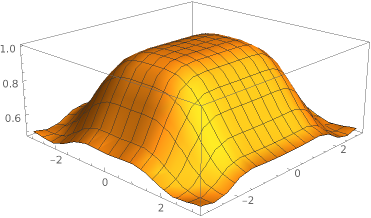
\includegraphics[scale=0.4]{d_dim_ex_1}
	\caption{$|\widehat{\phi}|$ on $(-\pi, \pi] \times (-\pi, \pi]$}
\end{figure}

\begin{itemize}
	\item $\sup|\widehat{\phi}| = 1$ and $\Omega(\phi)= \{\xi_0 \}  = \{ (0,0) \} $
	\begin{equation*}
	\Gamma_{0}(\xi)=-i\left(\frac{\tau^2}{24}-\frac{\tau\zeta^2}{96} +\frac{ \zeta^4}{96}\right) + \text{ h.o.t.}
	\end{equation*}
	
	\item $\mu_\phi = 1/2 + 1/4 = 3/4$
\end{itemize}
\end{frame}




\begin{frame}
\frametitle{Global decay estimate for $\abs{\phi^{(n)}}$: In $d$ dimensions}

Let $K = [-300,300]\times[-300,300]$ and pick $C=2$.  
\begin{equation*}
f(n)\coloneqq\max_{K}\abs{\phi^{(n)}}\leq 2n^{-\mu_\phi}= 2n^{-3/4}
\end{equation*}

\begin{figure}[!htb]
	\vspace{-10pt}
	\begin{subfigure}{0.49\textwidth}
		\centering
		\includegraphics[width=\textwidth]{Fig7a.eps}
		\caption{$\log_2 f(n)$, $\log_2 2n^{-3/4}$ vs $\log_2 n$.}
	\end{subfigure}
	\begin{subfigure}{0.49\textwidth}
		\centering
		\includegraphics[width=\textwidth]{Fig7b.eps}
		\caption{$f(n)$, $2n^{-3/4}$ vs. $n$}
	\end{subfigure}
	\label{fig:Conv_Pwr_2}
\end{figure}

\end{frame}



%%%%%%%%%%%%%%%%%%%%%%%%%%%%%%%


\begin{frame}
\frametitle{Global decay estimate for $\abs{\phi^{(n)}}$: In $d$ dimensions}

\underline{Example}:  $\phi: \mathbb{Z}^2 \to \mathbb{C}$ defined by $\phi=2^{-7}\phi_1-i2^{-11}\phi_2+2^{-21}\phi_3$ where

\scriptsize
\begin{equation*}
\phi_1(x,y)=\begin{cases}
15 + 15i &(x,y) = (\pm 1,0)\\
16 + 16i &(x,y) = (0, \pm 1)\\
1 + 1i &(x,y) = (\pm 3,0)\\
0 &\mbox{otherwise}
\end{cases},
\quad
\phi_2(x,y) = 
\begin{cases}
682 &(x,y) = (0,0)\\
152  &(x,y) = (\pm 2,0)\\
-28  &(x,y) = (\pm 4,0)\\
8 &(x,y) = (\pm 6, 0)\\
-1 &(x,y) = (\pm 8, 0)\\
60  &(x,y) = (0, \pm 2)\\
-24 &(x,y) = (0,\pm 4)\\
4 &(x,y) = (0,\pm 6)\\
0 &\mbox{otherwise}
\end{cases},
\end{equation*}
\begin{equation*}
\phi_3(x,y) = 
\begin{cases}
1387004 &(x,y) = (0,0)\\
-106722 &(x,y) = (\pm 2,0)\\
3960 &(x,y) = (\pm 4,0)\\
-1045 &(x,y) = (\pm 6, 0)\\
138  &(x,y) = (\pm 8, 0)\\
-9 &(x,y) = (\pm 10, 0)\\
-131072 &(x,y) = (0, \pm 2)\\
0 &\mbox{otherwise}
\end{cases}
\end{equation*}



\end{frame}



\begin{frame}
\frametitle{Global decay estimate for $\abs{\phi^{(n)}}$: In $d$ dimensions}



\begin{figure}
\begin{subfigure}{0.495\textwidth}
	\centering
	\includegraphics[width=\textwidth]{Fig10a.eps}
\end{subfigure}
\begin{subfigure}{0.495\textwidth}
	\centering
	\includegraphics[width=\textwidth]{Fig10b.eps}
\end{subfigure}
\end{figure}

\end{frame}





\begin{frame}
\frametitle{Global decay estimate for $\abs{\phi^{(n)}}$: In $d$ dimensions}

\begin{figure}
\vspace{-10pt}
\centering
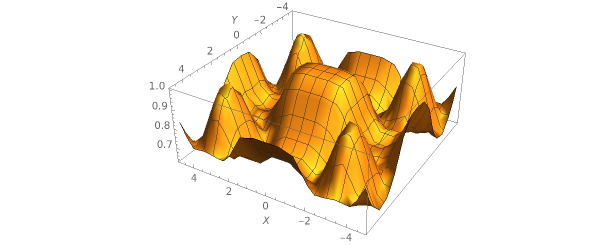
\includegraphics[scale=0.4]{d_dim_ex_2}
\caption{$|\widehat{\phi}|$ on $(-\pi, \pi] \times (-\pi, \pi]$}
\end{figure}
\begin{itemize}
\item $\sup|\widehat{\phi}| = 1$ and $\Omega(\phi)= \{\xi_0,\xi_1 \}  = \{ (0,0), (\pi,\pi) \} $
\begin{equation*}
\Gamma_{0}(\xi)=-i\left(\frac{\tau^6}{128}+\frac{\zeta^2}{8}\right) + \dots \qquad \Gamma_{1}(\xi)= +i\left(\frac{3\tau^2}{8}+\frac{\zeta^2}{4}\right) + \dots
\end{equation*}

\item $\mu_\phi = \min\{1/6+1/2, 1/2+1/2\} = \min\{2/3,1\}=  2/3$
\end{itemize}
\end{frame}




\begin{frame}
\frametitle{Global decay estimate for $\abs{\phi^{(n)}}$: In $d$ dimensions}

Let $K = [-500,500]\times[-500,500]$ and pick $C=1$.  
\begin{equation*}
f(n)\coloneqq\max_{K}\abs{\phi^{(n)}}\leq n^{-\mu_\phi}= n^{-2/3}
\end{equation*}
\begin{figure}[!htb]
\vspace{-10pt}
\begin{subfigure}{0.49\textwidth}
\centering
\includegraphics[width=\textwidth]{Fig9a.eps}
\caption{$\log_2 f(n)$, $\log_2 n^{-2/3}$ vs $\log_2 n$.}
\end{subfigure}
\begin{subfigure}{0.49\textwidth}
\centering
\includegraphics[width=\textwidth]{Fig9b.eps}
\caption{$f(n)$, $n^{-2/3}$ vs. $n$}
\end{subfigure}
\label{fig:Conv_Pwr_3}
\end{figure}

\end{frame}



\begin{frame}
\frametitle{Applications?}

\begin{enumerate}
	\item Numerical solutions to PDEs
	\begin{itemize}
		\item Approximate solutions by taking convolution powers\\
		$\,$\\
	\end{itemize}

\pause
	\item Quantum (field) theory
	\begin{itemize}
		\item Oscillatory integrals are ubiquitous
		\item Solutions to PDEs in QFT are often difficult to obtain/approximate\\
		$\,$\\
	\end{itemize}

\pause
	\item $\dots$\\
	$\,$\\
	
\pause

	\item For its own sake
	\begin{itemize}
		\item Inspiration from examples/numerical evidence
	\end{itemize}
\end{enumerate}

\end{frame}



\begin{frame}
\frametitle{What's next?}


\textbf{Classical result} (for probability distributions):

\begin{figure}
	\vspace{-10pt}
	\begin{subfigure}{0.27\textwidth}
		\centering
		\includegraphics[width=\textwidth]{convolve_22.eps}
	\end{subfigure}
\textcolor{black}{$\phi^{(n)}$ $\to$\text{ Gaussian}}
	\begin{subfigure}{0.27\textwidth}
		\centering
		\includegraphics[width=\textwidth]{gauss2d.eps}
	\end{subfigure}
\end{figure}


\pause

\textbf{\textcolor{magenta}{New conjecture:}} No positivity? No problem.

\begin{figure}
	\vspace{-10pt}
	\begin{subfigure}{0.35\textwidth}
		\centering
		\includegraphics[width=\textwidth]{Real_1500.eps}
	\end{subfigure}
$\quad$$\phi^{(n)}$ $\to$ $H^{iP}_t$$\quad$
	\begin{subfigure}{0.35\textwidth}
		\centering
		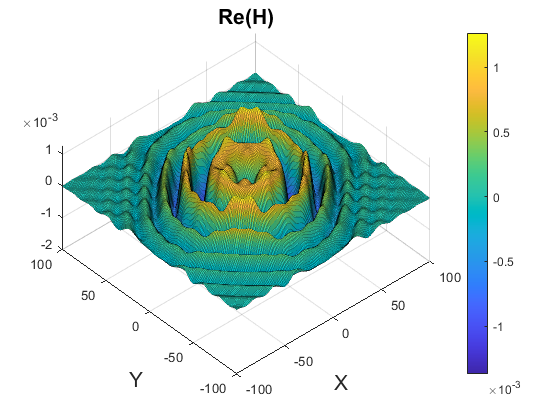
\includegraphics[width=\textwidth, trim={0 0 2.5cm 0},clip]{H_ex0.png}
	\end{subfigure}
\end{figure}
\end{frame}









\begin{frame}
\frametitle{Global decay estimate for $\abs{\phi^{(n)}}$: Extra}


\textcolor{purple}{\textbf{Proof ingredients:}} \\

1/ A generalized polar-coordinate integration formula (see \cite{bui2021generalized})\\
2/ Van der Corput lemma

\begin{lemma}[Van der Corput lemma]
	Let $g\in C^1([a,b])$ be complex-valued and let $\Phi\in C^2([a,b])$ be real-valued such that $\Phi''(x) \neq 0$ for all $x\in [a,b]$. Then
	\begin{equation*}
	\abs{\int^b_a g(u) e^{i\Phi(u)}\,du} \leq \min \lc \frac{4}{\delta}, \frac{8}{\sqrt{\rho}}  \rc \lp \norm{g'}_1 + \norm{g}_\infty \rp,
	\end{equation*}
	where $\delta = \inf_{x\in [a,b]} \abs{\Phi'(x)}$ and $\rho = \inf_{x\in [a,b]} \abs{\Phi''(x)}$. 
\end{lemma}


\includegraphics[scale=0.06]{key}$\,\,\,$ Integration by parts to bring the \textbf{amplitude} $g$ out\\

\includegraphics[scale=0.06]{key}$\,\,\,$ Integral dominated by the slowly-varying part of the \textbf{phase} $\Phi$



\end{frame}











%%%%%%%%%%%%%%%%%%%%%%%%%%%%%%%%%%%%%%%%%%%%%%%%
%
%
%
%\section{The classical polar-coordinate integration formula}
%\begin{frame}
%\frametitle{The classical polar-coordinate integration formula}
%
%In $\mathbb{R}^3$. Use spherical coordinates when $f$ has radial symmetry.
%\begin{equation*}
%\int_{\mathbb{R}^3} f(x)\,dx = \int_{0}^\infty \int_{0}^{2\pi} \int_0^{\pi} f(r\eta(\theta,\phi)) r^2 \sin\theta \,d\theta\, d\phi \, dr.
%\end{equation*}
%
%In $\mathbb{R}^d$?
%\begin{align*}\label{eq:StandardPolarIntegrationFormula}
%\int_{\mathbb{R}^d}f(x)\,dx=\int_{\mathbb{S}}\int_0^\infty f(r\eta)r^{d-1}\,dr\,\Theta(d\eta)=\int_0^\infty\int_\mathbb{S}f(r\eta)\Theta(d\eta)r^{d-1}\,dr,
%\end{align*}
%where
%\begin{align*}
%&\Theta\text{ is the spherical measure}
%&\quad\underbrace{\Theta(\mathbb{S})}_{\text{``Area''}} = d \cdot \underbrace{m(\mathbb{B})}_{\text{``Volume''}}
%\end{align*}
%\textbf{What if the symmetry of $f$ is anisotropic in $r$?}\\
%
%
%\end{frame}





%\begin{frame}
%\frametitle{A generalized polar-coordinate integration formula}
%
%\underline{Example:} $\mathbb{S}$ is replaced by  $S = \{ (\eta_1 ,\eta_2)\in \mathbb{R}^2 : P(\eta_1,\eta_2) = \eta_1^2 + \eta_2^4 = 1 \}$.\\
%$\,$ \\
%
%
%Any point $x\in \mathbb{R}^d\setminus \{ 0 \}$, can be written uniquely as $x = r^E \eta$, where $E = \text{diag}(1/2, 1/4)$ in the standard basis and $r> 0$.  \\
%$\,$\\
%
%
%$P$ is ``homogeneous'' with respect to $E$: $P(r^E\eta) = rP(\eta)$. \\
%$\,$\\
%
%
%$P$ is positive definite: $P \geq 0$ and $P(x) = 0 \iff x=0$. \\
%$\,$\\
%
%
%$E$ is not unique. For any $E$ such that $P(r^E\eta) = rP(\eta)$, we say that $E\in \text{Exp}(P)$. \\
%$\,$\\
%
%Can generalize this to define \textbf{positive homogeneous functions}.
%
%
%\end{frame}












%
%\begin{frame}
%\frametitle{Positive homogeneous functions}
%\begin{figure}[!htb]
%	\centering
%	\hspace{10pt}
%	\begin{subfigure}{0.5\textwidth}
%		\centering
%		\includegraphics[width=0.75\textwidth]{Fig2a.eps}
%		\vspace{-10pt}
%		\includegraphics[width=0.75\textwidth]{Fig2b.eps}
%		%\caption{}
%		%\label{fig:WeierstrassP_levelsets}
%	\end{subfigure}%
%	\hspace{-30pt}
%	\begin{subfigure}{0.5\textwidth}
%		\centering
%		\includegraphics[width=0.75\textwidth]{Fig2c.eps}
%		\vspace{-10pt}
%		\includegraphics[width=0.75\textwidth]{Fig2d.eps}
%		%\caption{}
%		%\label{fig:Q_levelsets}
%	\end{subfigure}
%	\caption{The graphs of $P$, $Q$ with associated $S_P$, $S_Q$, $B_P$, $B_Q$. Here, $Q(x,y) = \abs{(x,y)}$. $P$ is $Q$ multiplied by a version of the Weierstrass function. }
%	\label{fig:Weierstrass}
%\end{figure}
%\end{frame}

%
%
%\begin{frame}
%\frametitle{Positive homogeneous functions}
%\underline{More results and definitions}:
%\begin{itemize}
%	\item Let $\text{Sym}(P)$ denote the set of $O\in\text{End}(\mathbb{R}^d)$ for which
%	\begin{equation*}
%	P(Ox)=P(x)
%	\end{equation*}
%	$\text{Sym}(P)$ is a subgroup of $O(\mathbb{R}^d)$.
%	
%	\item $\text{Exp}(P) = O^* \text{Exp}(P) O$ for any $O\in \text{Sym}(P)$.
%	
%	
%	\item $\tr E>0$ for any $E\in \text{Exp}(P)$, $P$ positive homogeneous.
%	
%	\item \textbf{Subhomogeneous \& strongly subhomogeneous} functions wrt $E$.
%\end{itemize}
%\end{frame}
%
%
%\begin{frame}
%\frametitle{Positive homogeneous functions}
%\begin{definition}\label{def:homogeneous_types}
%	$Q$ is continuous and complex-valued, defined on an open nbh $\mathcal{O}$ of $0$ in $\mathbb{R}^d$. $E\in\text{End}(\mathbb{R}^d)$ is such that $\{r^E\}$ is contracting.
%	\begin{enumerate}
%		\item We say that $Q$ is \textbf{subhomogeneous with respect to $E$} if, for each $\epsilon>0$ and compact set $K\subseteq\mathbb{R}^d$, there is a $\delta>0$ for which
%		\begin{equation*}
%		\abs{Q(r^E\xi)}\leq \epsilon r, \quad \forall 0<r<\delta, \xi\in K
%		\end{equation*}
%
%		\item Given $k\geq 1$, we say that $Q$ is \textbf{strongly subhomogeneous with respect to $E$ of order $k$} if $Q\in C^k(\mathcal{O})$ and, for each $\epsilon>0$ and compact set $K\subseteq\mathbb{R}^d$, there is a $\delta>0$ for which
%		\begin{equation*}
%		\abs{r^j\partial_r^j Q(r^E\xi)}\leq \epsilon r, \quad \forall j=1,2,\dots,k, 0<r<\delta, \xi\in K.
%		\end{equation*}
%	\end{enumerate}
%\end{definition}
%
%\end{frame}
%
%
%
%\begin{frame}
%\frametitle{A generalized polar-coordinate integration formula}
%
%If $S$ is smooth, can construct the formula from smooth manifold theory.\\
%$\,$\\
%
%
%For generic $S$, however, we need measure theory:
%\begin{itemize}
%	\item Construct $\sigma_{P,E}$, a surface measure on $S$
%	\item Construct the integration formula from $\sigma_{P,E}$
%	\item Show that the constructions don't depend on $E$ (makes sense)
%\end{itemize}
%
%\end{frame}
%
%
%\begin{frame}
%\frametitle{A generalized polar-coordinate integration formula}
%
%
%
%\end{frame}
%
%
%
%









%%%%%%%%%%%%%%%%%%%%%%%%%%%%%%%%%%%%%%%%%%%%%%%%%%%
%%%%%%%%%%%%%%%%%%%%%%%%%%%%%%%%%%%%%%%%%%%%%%%%%%%
%%%%%%%%%%%%%%%%%%%%%%%%%%%%%%%%%%%%%%%%%%%%%%%%%%%
%%%%%%%%%%%%%%%%%%%%%%%%%%%%%%%%%%%%%%%%%%%%%%%%%%%
%%%%%%%%%%%%%%%%%%%%%%%%%%%%%%%%%%%%%%%%%%%%%%%%%%%
%%%%%%%%%%%%%%%%%%%%%%%%%%%%%%%%%%%%%%%%%%%%%%%%%%%


\begin{frame}
\frametitle{References}
\bibliographystyle{amsalpha}
\bibliography{GPIF}{}
\end{frame}



\end{document}
